%%%%%%%%%%%%%%%%%%%%%%%%%%%%%%%%%%%%%%%%%%%%%%%%%%%%%%%%%%%%%%%%%%%%%%%%%%%%%%%
\section{Context \& Motivations}
%%%%%%%%%%%%%%%%%%%%%%%%%%%%%%%%%%%%%%%%%%%%%%%%%%%%%%%%%%%%%%%%%%%%%%%%%%%%%%%


%%%%%%%%%%%%%%%%%%%%%%%%%%%%%%%%%%%%%%%%%%%%%%%%%%%%%%%%%%%%%%%%%%%%%%%%%%%%%%%
\begin{frame}{Machine Learning Models are now used everywhere}
%%%%%%%%%%%%%%%%%%%%%%%%%%%%%%%%%%%%%%%%%%%%%%%%%%%%%%%%%%%%%%%%%%%%%%%%%%%%%%%

  \begin{minipage}{\textwidth}
    \centering
    In the last 10 years, Machine Learning models have been deployed \\ in many \orangebold{day-to-day applications}.
  \end{minipage}

  \vspace{0.5cm}

  \begin{table}
    \footnotesize{
      \centering
      \begin{tabular}{
	cccc
      }
	\begin{minipage}{0.22\textwidth}
	  \centering
	  
\includegraphics[width=0.40\textwidth]{images/icons/www.pdf}
	\end{minipage}
	& 
	\begin{minipage}{0.22\textwidth}
	  \centering
	  
\includegraphics[width=0.40\textwidth]{images/icons/translate.pdf}
	\end{minipage}
	&
	\begin{minipage}{0.22\textwidth}
	  \centering
	  
\includegraphics[width=0.33\textwidth]{images/icons/assistant-vocal.pdf}
	\end{minipage}
	& 
	\begin{minipage}{0.22\textwidth}
	  \centering
	  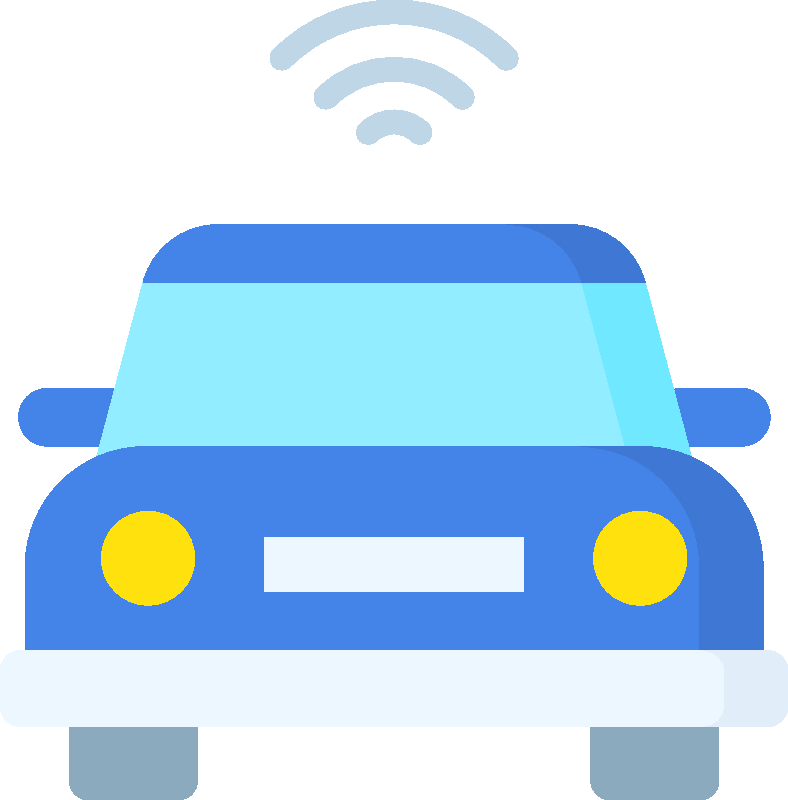
\includegraphics[width=0.40\textwidth]{images/icons/autonomous-car.pdf}
	\end{minipage} \\[0.5cm]
	Web Search & Translation & Vocal Assistants & Self-driving cars
      \end{tabular}
    }
  \end{table}

  \vspace{0.4cm}
  \visible<2->{Machine Learning models have a growing impact on society as more and more are \orangebold{deployed into critical-systems}: weapons, justice, healthcare, etc.}


\end{frame}



% %%%%%%%%%%%%%%%%%%%%%%%%%%%%%%%%%%%%%%%%%%%%%%%%%%%%%%%%%%%%%%%%%%%%%%%%%%%%%%%
% \begin{frame}{Supervised Learning}
% %%%%%%%%%%%%%%%%%%%%%%%%%%%%%%%%%%%%%%%%%%%%%%%%%%%%%%%%%%%%%%%%%%%%%%%%%%%%%%%
%
%   \only<1>{
%     \begin{tabular}{cc}
%       \begin{minipage}[t]{0.48\textwidth}
% 	\centering
% 	Images $\xvec \in \Xcal \subset \Rbb^d$
%       \end{minipage} & 
%       \begin{minipage}[t]{0.48\textwidth}
% 	\centering
% 	\vphantom{
% 	\textbf{Goal}: find a function $h$}
%       \end{minipage}
%     \end{tabular}
%   }
%   \only<2->{
%     \begin{tabular}{cc}
%       \begin{minipage}[t]{0.48\textwidth}
% 	\centering
% 	Images $\xvec \in \Xcal \subset \Rbb^d$
%       \end{minipage} & 
%       \begin{minipage}[t]{0.48\textwidth}
% 	\centering
% 	\textbf{Goal}: find a function $h$
%       \end{minipage}
%     \end{tabular}
%   }
%   \begin{minipage}{0.45\textwidth}
%     \centering
%     
\includegraphics[scale=0.25]{./images/animals/animals.pdf}
%   \end{minipage}
%   \hfill
%   \begin{minipage}{0.15\textwidth}
%     \visible<2->{$\Rightarrow$}
%   \end{minipage}
%   \hfill
%   \begin{minipage}{0.38\textwidth}
%     \flushleft
%     \only<2>{$ \displaystyle h \Bigg( \quad \quad \quad \Bigg)  = \text{``elephant''}$}
%     \only<3>{$ \displaystyle h \Bigg( \quad \quad \quad \Bigg)  = \text{``bird''}$}
%     \only<4>{$ \displaystyle h \Bigg( \quad \quad \quad \Bigg)  = \text{``frog''}$}
%     \only<5->{$ \displaystyle h \Bigg( \quad \quad \quad \Bigg)  = \text{``squirrel''}$}
%     \begin{tikzpicture}[overlay]
%       \only<2>{\node [anchor=north east, xshift=-2.5cm, yshift=0.6cm]
% 	{ 
\includegraphics[scale=0.07]{./images/animals/elephant.pdf} };}
%       \only<3>{\node [anchor=north east, xshift=-1.8cm, yshift=0.6cm]
% 	{ 
\includegraphics[scale=0.07]{./images/animals/bird.pdf} };}
%       \only<4>{\node [anchor=north east, xshift=-1.7cm, yshift=0.6cm]
% 	{ 
\includegraphics[scale=0.07]{./images/animals/frog.pdf} };}
%       \only<5->{\node [anchor=north east, xshift=-2cm, yshift=0.6cm]
% 	{ 
\includegraphics[scale=0.07]{./images/animals/squirrel.pdf} };}
%       \only<6->{
% 	\node [anchor=north east, xshift=-2.8cm, yshift=-0.7cm] {$\xvec \in \Xcal$};
% 	\node [anchor=north east, xshift=-0.3cm, yshift=-0.7cm] {$y \in \Ycal$};
% 	\path[->] (-2.8, -1.0) edge [out=0, in=-90] (-2.4, -0.6);
% 	\path[->] (-0.8, -0.7) edge [bend right] (-0.8, -0.1);
%       }
%     \end{tikzpicture}
%   \end{minipage}
%
%   \vspace{0.2cm}
%   {\small
%     \begin{itemize}
%       \item[$\bullet$]<6-> \textbf{Assumption:} ground-truth distribution $\Dcal$ describing the relation $\Xcal$ and $\Ycal$
%       \item[$\bullet$]<7-> Define an hypothesis space $h \in \Hcal$ and a loss function $\ell: \Ycal \times \Ycal \rightarrow \Rbb^{+}$
%       \item<8->
%       \vspace{-0.2cm}
%       \begin{equation}
% 	R(h) \triangleq \E_{(\xvec, y) \in \Dcal} \ell \big( h(\xvec), y \big) \quad \quad \quad \quad h^* = \argmin_{h \in \Hcal} R(h)
%       \end{equation}
%       \item[$\bullet$]<9-> In practice, we only have access to a finite set of training samples, $\{(\xvec_i, y_i)\}_{i \in [m]}$
%       \item<9->
%       \vspace{-0.2cm}
%       \begin{equation}
%         \hat{R}_m(h) \triangleq \frac{1}{m} \sum_{i=1}^{m} \ell \big(h(\xvec_i), y_i \big)  \visible<10->{\quad + \underbrace{r(h)}_{\text{penalty term}}}
%       \end{equation}
%       \item[$\bullet$]<10-> We can favor an hypothesis by adding a penalty term
%     \end{itemize}
%   }
%
%
% \end{frame}



%%%%%%%%%%%%%%%%%%%%%%%%%%%%%%%%%%%%%%%%%%%%%%%%%%%%%%%%%%%%%%%%%%%%%%%%%%%%%%%
\begin{frame}{Supervised Learning}
%%%%%%%%%%%%%%%%%%%%%%%%%%%%%%%%%%%%%%%%%%%%%%%%%%%%%%%%%%%%%%%%%%%%%%%%%%%%%%%

  \only<1>{
    \begin{tabular}{cc}
      \begin{minipage}[t]{0.48\textwidth}
	\centering
	Images $\xvec \in \Xcal \subset \Rbb^d$
      \end{minipage} & 
      \begin{minipage}[t]{0.48\textwidth}
	\centering
	\vphantom{
	\textbf{Goal}: find a function $h$}
      \end{minipage}
    \end{tabular}
  }
  \only<2->{
    \begin{tabular}{cc}
      \begin{minipage}[t]{0.48\textwidth}
	\centering
	Images $\xvec \in \Xcal \subset \Rbb^d$
      \end{minipage} & 
      \begin{minipage}[t]{0.48\textwidth}
	\centering
	\textbf{Goal}: find a function $h$
      \end{minipage}
    \end{tabular}
  }
  \begin{minipage}{0.45\textwidth}
    \centering
    
\includegraphics[scale=0.25]{./images/animals/animals.pdf}
  \end{minipage}
  \hfill
  \begin{minipage}{0.15\textwidth}
    \visible<2->{$\Rightarrow$}
  \end{minipage}
  \hfill
  \begin{minipage}{0.38\textwidth}
    \flushleft
    \visible<2->{$ \displaystyle h \Bigg( \quad \quad \quad \Bigg)  = \text{``elephant''}$}
    \begin{tikzpicture}[overlay]
      \visible<2->{\node [anchor=north east, xshift=-2.2cm, yshift=0.6cm] (elephant) { 
           
\includegraphics[scale=0.07]{./images/animals/elephant.pdf} };
	\node [anchor=north east, xshift=-2.9cm, yshift=-0.7cm] (Xset) {$\xvec \in \Xcal$};
	\node [anchor=north east, xshift=-0.3cm, yshift=-0.7cm] (Yset) {$y \in \Ycal$};
        \path[->] (Xset.east) edge [bend right] (elephant.south);
	\path[->] (-0.8, -0.7) edge [bend right] (-0.8, -0.1);
      }
    \end{tikzpicture}
  \end{minipage}

  \vspace{0.2cm}
  {\small
    \begin{itemize}
      \item[$\bullet$]<3-> \textbf{Assumption:} ground-truth distribution $\Dcal$ describing the relation between $\Xcal$ and $\Ycal$
      \item[$\bullet$]<4-> Define a hypothesis space $\Hcal$ and a loss function $\ell: \Ycal \times \Ycal \rightarrow \Rbb^{+}$
      \item<5->
      \vspace{-0.2cm}
      \begin{equation}
	R(h) \triangleq \E_{(\xvec, y) \in \Dcal} \ell \big( h(\xvec), y \big) \quad \quad \quad \quad h^* = \argmin_{h \in \Hcal} R(h)
      \end{equation}
      \item[$\bullet$]<6-> In practice, we only have access to a finite set of training samples, $\{(\xvec_i, y_i)\}_{i \in [m]}$
      \item<6->
      \vspace{-0.2cm}
      \begin{equation}
        \hat{R}_m(h) \triangleq \frac{1}{m} \sum_{i=1}^{m} \ell \big(h(\xvec_i), y_i \big)  \visible<7->{\quad + \underbrace{P(h)}_{\text{penalty term}}}
      \end{equation}
      \item[$\bullet$]<7-> We add a penalty term to control the choice of the hypothesis
    \end{itemize}
  }


\end{frame}







% %%%%%%%%%%%%%%%%%%%%%%%%%%%%%%%%%%%%%%%%%%%%%%%%%%%%%%%%%%%%%%%%%%%%%%%%%%%%%%%
% \begin{frame}{Feedfoward Neural Networks}
% %%%%%%%%%%%%%%%%%%%%%%%%%%%%%%%%%%%%%%%%%%%%%%%%%%%%%%%%%%%%%%%%%%%%%%%%%%%%%%%
%
%   A Feedfoward Neural Neural, example:
%   $h(\xvec) = \only<9->{\phi^{(4)} \circ} \only<8->{\phi^{(3)} \circ} \phi^{(2)} \circ \phi^{(1)}(\xvec)$
%
%   \vspace{-0.2cm}
%   \only<1>{
%     \begin{minipage}{\textwidth}
%       \centering
%       \begin{overpic}[scale=0.2]{images/icons/neural_network_1.pdf}
%        \put (-13,31) {
% 	 \begin{minipage}{0.3\textwidth}
% 	    \begin{itemize}[parsep=0pt,itemsep=0pt]
% 	      \item[{
\includegraphics[trim=4mm 11mm 0 0,clip,scale=0.1,valign=c]{images/icons/image.pdf}}] \footnotesize{Images}
% 	      \item[{
\includegraphics[trim=4mm 11mm 0 0,clip,scale=0.1,valign=c]{images/icons/sound.pdf}}] \footnotesize{Sounds}
% 	      \item[{
\includegraphics[trim=0mm 11mm 0 0,clip,scale=0.014,valign=c]{images/icons/text.pdf}}] \footnotesize{Texts}
% 	    \end{itemize}
% 	 \end{minipage}
%        }
%        \put (75,31) {
% 	 \begin{minipage}{0.1\textwidth}
% 	   \footnotesize{Outputs}
% 	 \end{minipage}
%        }
%       \end{overpic}
%     \end{minipage}
%   }
%   \only<2-4>{
%     \begin{minipage}{\textwidth}
%       \centering
%       \begin{overpic}[scale=0.2]{images/icons/neural_network_1.pdf}
%        \put (-13,31) {
% 	 \begin{minipage}{0.3\textwidth}
% 	    \begin{itemize}[parsep=0pt,itemsep=0pt]
% 	      \item[{
\includegraphics[trim=4mm 11mm 0 0,clip,scale=0.1,valign=c]{images/icons/image.pdf}}] \footnotesize{Images}
% 	      \item[{
\includegraphics[trim=4mm 11mm 0 0,clip,scale=0.1,valign=c]{images/icons/sound.pdf}}] \footnotesize{Sounds}
% 	      \item[{
\includegraphics[trim=0mm 11mm 0 0,clip,scale=0.014,valign=c]{images/icons/text.pdf}}] \footnotesize{Texts}
% 	    \end{itemize}
% 	 \end{minipage}
%        }
%        \put (75,31) {
% 	 \begin{minipage}{0.1\textwidth}
% 	   \footnotesize{Outputs}
% 	 \end{minipage}
%        }
%        \put (42,19) {
% 	\begin{tikzpicture}
% 	  \draw[color=OrangePSL, thick] (0,0) -- (0.5,0) -- (0.5,1.3) -- (0,1.3) -- (0,0);
% 	\end{tikzpicture}
%        }
%        \put (42,51) {
% 	 \orangebold{\footnotesize{Layer}}
%        }
%       \end{overpic}
%     \end{minipage}
%   }
%   \only<5>{
%     \begin{minipage}{\textwidth}
%       \centering
%       \begin{overpic}[scale=0.2]{images/icons/neural_network_1.pdf}
%        \put (-13,31) {
% 	 \begin{minipage}{0.3\textwidth}
% 	    \begin{itemize}[parsep=0pt,itemsep=0pt]
% 	      \item[{
\includegraphics[trim=4mm 11mm 0 0,clip,scale=0.1,valign=c]{images/icons/image.pdf}}] \footnotesize{Images}
% 	      \item[{
\includegraphics[trim=4mm 11mm 0 0,clip,scale=0.1,valign=c]{images/icons/sound.pdf}}] \footnotesize{Sounds}
% 	      \item[{
\includegraphics[trim=0mm 11mm 0 0,clip,scale=0.014,valign=c]{images/icons/text.pdf}}] \footnotesize{Texts}
% 	    \end{itemize}
% 	 \end{minipage}
%        }
%        \put (75,31) {
% 	 \begin{minipage}{0.1\textwidth}
% 	   \footnotesize{Outputs}
% 	 \end{minipage}
%        }
%       \end{overpic}
%     \end{minipage}
%   }
%   \only<6>{
%     \begin{minipage}{\textwidth}
%       \centering
%       \begin{overpic}[scale=0.2]{images/icons/neural_network_2.pdf}
% 	\put (-13,31) {
% 	 \begin{minipage}{0.3\textwidth}
% 	    \begin{itemize}[parsep=0pt,itemsep=0pt]
% 	      \item[{
\includegraphics[trim=4mm 11mm 0 0,clip,scale=0.1,valign=c]{images/icons/image.pdf}}] \footnotesize{Images}
% 	      \item[{
\includegraphics[trim=4mm 11mm 0 0,clip,scale=0.1,valign=c]{images/icons/sound.pdf}}] \footnotesize{Sounds}
% 	      \item[{
\includegraphics[trim=0mm 11mm 0 0,clip,scale=0.014,valign=c]{images/icons/text.pdf}}] \footnotesize{Texts}
% 	    \end{itemize}
% 	 \end{minipage}
%        }
%        \put (75,31) {
% 	 \begin{minipage}{0.1\textwidth}
% 	   \footnotesize{Outputs}
% 	 \end{minipage}
%        }
%       \end{overpic}
%     \end{minipage}
%   }
%   \only<7>{
%     \begin{minipage}{\textwidth}
%       \centering
%       \begin{overpic}[scale=0.2]{images/icons/neural_network_3.pdf}
%        \put (-13,31) {
% 	 \begin{minipage}{0.3\textwidth}
% 	    \begin{itemize}[parsep=0pt,itemsep=0pt]
% 	      \item[{
\includegraphics[trim=4mm 11mm 0 0,clip,scale=0.1,valign=c]{images/icons/image.pdf}}] \footnotesize{Images}
% 	      \item[{
\includegraphics[trim=4mm 11mm 0 0,clip,scale=0.1,valign=c]{images/icons/sound.pdf}}] \footnotesize{Sounds}
% 	      \item[{
\includegraphics[trim=0mm 11mm 0 0,clip,scale=0.014,valign=c]{images/icons/text.pdf}}] \footnotesize{Texts}
% 	    \end{itemize}
% 	 \end{minipage}
%        }
%        \put (75,31) {
% 	 \begin{minipage}{0.1\textwidth}
% 	   \footnotesize{Outputs}
% 	 \end{minipage}
%        }
%       \end{overpic}
%     \end{minipage}
%   }
%   \only<8>{
%     \begin{minipage}{\textwidth}
%       \centering
%       \begin{overpic}[scale=0.2]{images/icons/neural_network_4.pdf}
%        \put (-25,31) {
% 	 \begin{minipage}{0.3\textwidth}
% 	    \begin{itemize}[parsep=0pt,itemsep=0pt]
% 	      \item[{
\includegraphics[trim=4mm 11mm 0 0,clip,scale=0.1,valign=c]{images/icons/image.pdf}}] \footnotesize{Images}
% 	      \item[{
\includegraphics[trim=4mm 11mm 0 0,clip,scale=0.1,valign=c]{images/icons/sound.pdf}}] \footnotesize{Sounds}
% 	      \item[{
\includegraphics[trim=0mm 11mm 0 0,clip,scale=0.014,valign=c]{images/icons/text.pdf}}] \footnotesize{Texts}
% 	    \end{itemize}
% 	 \end{minipage}
%        }
%        \put (90,31) {
% 	 \begin{minipage}{0.1\textwidth}
% 	   \footnotesize{Outputs}
% 	 \end{minipage}
%        }
%       \end{overpic}
%     \end{minipage}
%   }
%   \only<9>{
%     \begin{minipage}{\textwidth}
%       \centering
%       \begin{overpic}[scale=0.2]{images/icons/neural_network_5.pdf}
%         \put (-35,31) {
% 	 \begin{minipage}{0.3\textwidth}
% 	    \begin{itemize}[parsep=0pt,itemsep=0pt]
% 	      \item[{
\includegraphics[trim=4mm 11mm 0 0,clip,scale=0.1,valign=c]{images/icons/image.pdf}}] \footnotesize{Images}
% 	      \item[{
\includegraphics[trim=4mm 11mm 0 0,clip,scale=0.1,valign=c]{images/icons/sound.pdf}}] \footnotesize{Sounds}
% 	      \item[{
\includegraphics[trim=0mm 11mm 0 0,clip,scale=0.014,valign=c]{images/icons/text.pdf}}] \footnotesize{Texts}
% 	    \end{itemize}
% 	 \end{minipage}
%        }
%        \put (100,31) {
% 	 \begin{minipage}{0.1\textwidth}
% 	   \footnotesize{Outputs}
% 	 \end{minipage}
%        }
%       \end{overpic}
%     \end{minipage}
%   }
%
%   \vspace{-0.5cm}
%   \visible<2->{
%     each layer is defined as:
%     \begin{equation}
%       \phi^{(i)} \triangleq \xvec \mapsto 
% 	{\color<4>{OrangePSL}{\rho \big(}}
% 	\ {\color<3>{OrangePSL}{\Wmat^{(i)}}} \xvec + {\color<3>{OrangePSL}{\bvec^{(i)}}} \ 
% 	{\color<4>{OrangePSL}{\big)}}
%     \end{equation}
%     \vspace{-0.3cm}
%     {\small
%     \begin{itemize}
%       \visible<3->{\item[$\bullet$] Linear transform: the matrix $\Wmat^{(i)}$ and the $\bvec^{(i)}$ are the parameters.}
%       \visible<4->{\item[$\bullet$] Nonlinear function $\rho$ (\eg, Sigmoid, Tanh, Leaky-ReLU, etc.)}
%     \end{itemize}}
%   }
%
%   \begin{overlayarea}{\textwidth}{4cm}
%     \only<4>{
%       \begin{minipage}{\textwidth}
% 	\centering
% 	\begin{minipage}{0.32\textwidth}
% 	  \centering
% 	  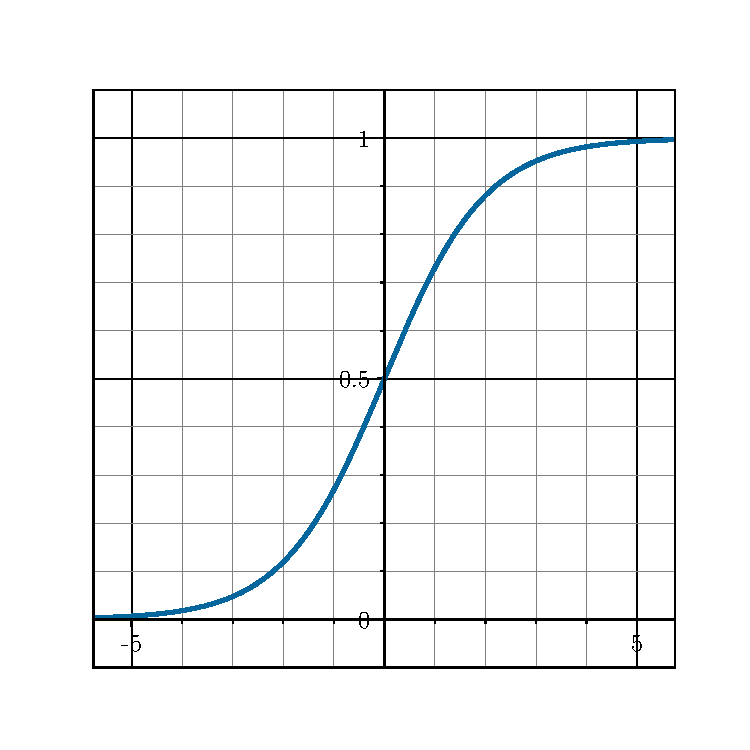
\includegraphics[scale=0.15]{images/nonlinear_func/sigmoid.pdf} \\
% 	  \tiny{Sigmoid Activation}
% 	\end{minipage}
% 	\hfill
% 	\begin{minipage}{0.32\textwidth}
% 	  \centering
% 	  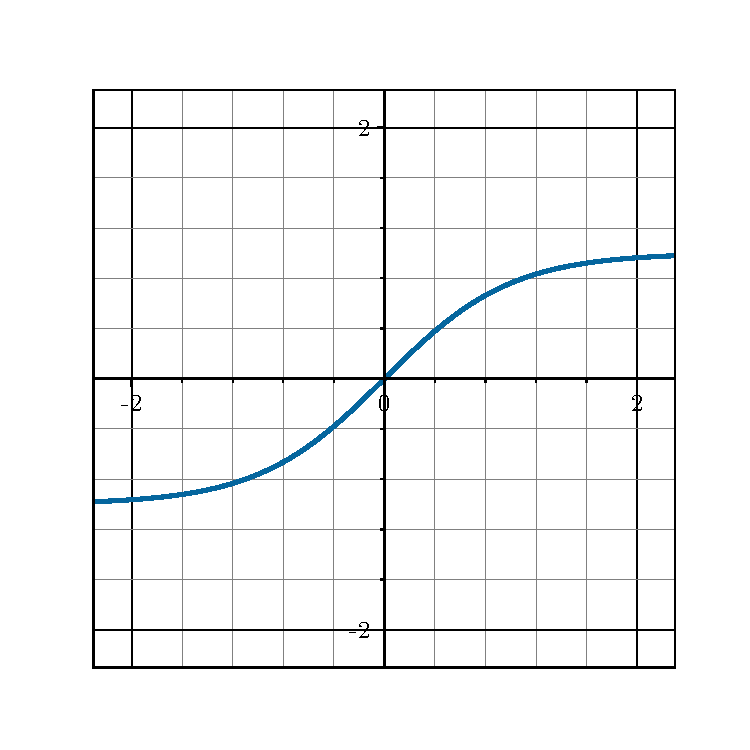
\includegraphics[scale=0.15]{images/nonlinear_func/tanh.pdf} \\
% 	  \tiny{Tanh Activation}
% 	\end{minipage}
% 	\hfill
% 	\begin{minipage}{0.31\textwidth}
% 	  \centering
% 	  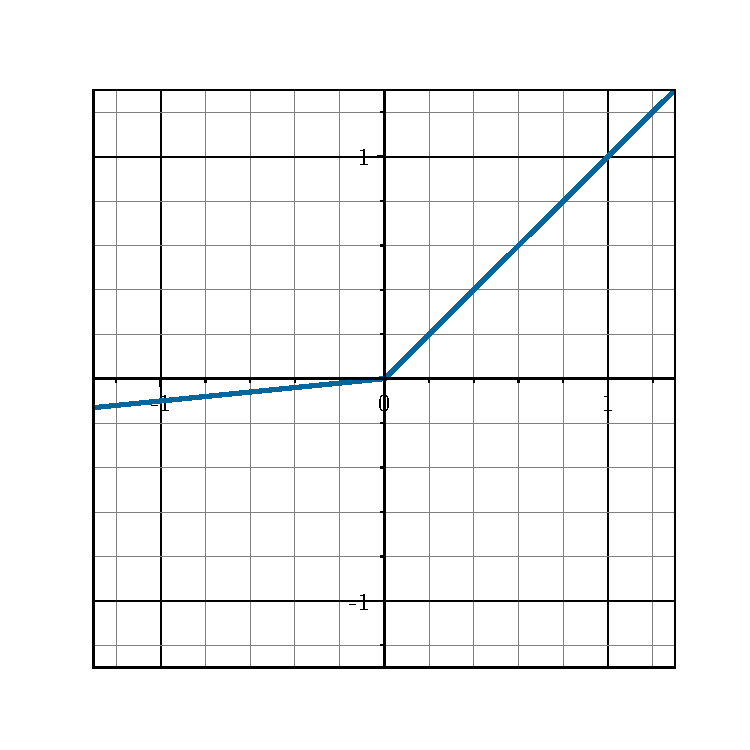
\includegraphics[scale=0.15]{images/nonlinear_func/relu.pdf} \\
% 	  \tiny{Leaky-ReLU Activation}
% 	\end{minipage}
%       \end{minipage}
%     }
%     \only<5->{
%       \begin{mdframed}[linecolor=OrangePSL,linewidth=1pt]
% 	\centering
% 	In general, increasing the number of parameters makes the network more \orangebold{expressive} and more \orangebold{accurate}.
%       \end{mdframed}
%     }
%   \end{overlayarea}
%
% \end{frame}




%%%%%%%%%%%%%%%%%%%%%%%%%%%%%%%%%%%%%%%%%%%%%%%%%%%%%%%%%%%%%%%%%%%%%%%%%%%%%%%
\begin{frame}{Feedfoward Neural Networks}
%%%%%%%%%%%%%%%%%%%%%%%%%%%%%%%%%%%%%%%%%%%%%%%%%%%%%%%%%%%%%%%%%%%%%%%%%%%%%%%

  A Feedfoward Neural Network:
  % $h(\xvec) = \only<7->{\phi^{(4)} \circ} \only<6->{\phi^{(3)} \circ} \phi^{(2)} \circ \phi^{(1)}(\xvec)$
  $h(\xvec) = \phi^{(p)} \circ \cdots \circ \phi^{(2)} \circ \phi^{(1)}(\xvec)$

  \vspace{-0.2cm}
  \only<1-3>{
    \begin{minipage}{\textwidth}
      \centering
      \begin{overpic}[scale=0.2]{images/icons/neural_network_1.pdf}
       \put (-13,31) {
	 \begin{minipage}{0.3\textwidth}
	    \begin{itemize}[parsep=0pt,itemsep=0pt]
	      \item[{
\includegraphics[trim=4mm 11mm 0 0,clip,scale=0.1,valign=c]{images/icons/image.pdf}}] \footnotesize{Images}
	      \item[{
\includegraphics[trim=4mm 11mm 0 0,clip,scale=0.1,valign=c]{images/icons/sound.pdf}}] \footnotesize{Sounds}
	      \item[{
\includegraphics[trim=0mm 11mm 0 0,clip,scale=0.014,valign=c]{images/icons/text.pdf}}] \footnotesize{Texts}
	    \end{itemize}
	 \end{minipage}
       }
       \put (75,31) {
	 \begin{minipage}{0.1\textwidth}
	   \footnotesize{Outputs}
	 \end{minipage}
       }
       \visible<2->{
	 \put (42,51) {
	   \orangebold{\footnotesize{Layer}}
	 }
	 \put (42,19) {
	  \begin{tikzpicture}
	    \draw[color=OrangePSL, thick] (0,0) -- (0.5,0) -- (0.5,1.3) -- (0,1.3) -- (0,0);
	  \end{tikzpicture}
	 }
       }
      \end{overpic}
    \end{minipage}
  }
  \only<4>{
    \begin{minipage}{\textwidth}
      \centering
      \begin{overpic}[scale=0.2]{images/icons/neural_network_2.pdf}
	\put (-13,31) {
	 \begin{minipage}{0.3\textwidth}
	    \begin{itemize}[parsep=0pt,itemsep=0pt]
	      \item[{
\includegraphics[trim=4mm 11mm 0 0,clip,scale=0.1,valign=c]{images/icons/image.pdf}}] \footnotesize{Images}
	      \item[{
\includegraphics[trim=4mm 11mm 0 0,clip,scale=0.1,valign=c]{images/icons/sound.pdf}}] \footnotesize{Sounds}
	      \item[{
\includegraphics[trim=0mm 11mm 0 0,clip,scale=0.014,valign=c]{images/icons/text.pdf}}] \footnotesize{Texts}
	    \end{itemize}
	 \end{minipage}
       }
       \put (75,31) {
	 \begin{minipage}{0.1\textwidth}
	   \footnotesize{Outputs}
	 \end{minipage}
       }
      \end{overpic}
    \end{minipage}
  }
  \only<5>{
    \begin{minipage}{\textwidth}
      \centering
      \begin{overpic}[scale=0.2]{images/icons/neural_network_3.pdf}
       \put (-13,31) {
	 \begin{minipage}{0.3\textwidth}
	    \begin{itemize}[parsep=0pt,itemsep=0pt]
	      \item[{
\includegraphics[trim=4mm 11mm 0 0,clip,scale=0.1,valign=c]{images/icons/image.pdf}}] \footnotesize{Images}
	      \item[{
\includegraphics[trim=4mm 11mm 0 0,clip,scale=0.1,valign=c]{images/icons/sound.pdf}}] \footnotesize{Sounds}
	      \item[{
\includegraphics[trim=0mm 11mm 0 0,clip,scale=0.014,valign=c]{images/icons/text.pdf}}] \footnotesize{Texts}
	    \end{itemize}
	 \end{minipage}
       }
       \put (75,31) {
	 \begin{minipage}{0.1\textwidth}
	   \footnotesize{Outputs}
	 \end{minipage}
       }
      \end{overpic}
    \end{minipage}
  }
  \only<6>{
    \begin{minipage}{\textwidth}
      \centering
      \begin{overpic}[scale=0.2]{images/icons/neural_network_4.pdf}
       \put (-25,31) {
	 \begin{minipage}{0.3\textwidth}
	    \begin{itemize}[parsep=0pt,itemsep=0pt]
	      \item[{
\includegraphics[trim=4mm 11mm 0 0,clip,scale=0.1,valign=c]{images/icons/image.pdf}}] \footnotesize{Images}
	      \item[{
\includegraphics[trim=4mm 11mm 0 0,clip,scale=0.1,valign=c]{images/icons/sound.pdf}}] \footnotesize{Sounds}
	      \item[{
\includegraphics[trim=0mm 11mm 0 0,clip,scale=0.014,valign=c]{images/icons/text.pdf}}] \footnotesize{Texts}
	    \end{itemize}
	 \end{minipage}
       }
       \put (90,31) {
	 \begin{minipage}{0.1\textwidth}
	   \footnotesize{Outputs}
	 \end{minipage}
       }
      \end{overpic}
    \end{minipage}
  }
  \only<7>{
    \begin{minipage}{\textwidth}
      \centering
      \begin{overpic}[scale=0.2]{images/icons/neural_network_5.pdf}
        \put (-35,31) {
	 \begin{minipage}{0.3\textwidth}
	    \begin{itemize}[parsep=0pt,itemsep=0pt]
	      \item[{
\includegraphics[trim=4mm 11mm 0 0,clip,scale=0.1,valign=c]{images/icons/image.pdf}}] \footnotesize{Images}
	      \item[{
\includegraphics[trim=4mm 11mm 0 0,clip,scale=0.1,valign=c]{images/icons/sound.pdf}}] \footnotesize{Sounds}
	      \item[{
\includegraphics[trim=0mm 11mm 0 0,clip,scale=0.014,valign=c]{images/icons/text.pdf}}] \footnotesize{Texts}
	    \end{itemize}
	 \end{minipage}
       }
       \put (100,31) {
	 \begin{minipage}{0.1\textwidth}
	   \footnotesize{Outputs}
	 \end{minipage}
       }
      \end{overpic}
    \end{minipage}
  }

  \vspace{-0.5cm}
  \visible<2->{
    each layer is defined as:
    \begin{equation}
      \phi^{(i)} \triangleq \xvec \mapsto 
	\rho \big(
	\ \Wmat^{(i)} \xvec + \bvec^{(i)} \ 
	\big)
    \end{equation}
    \vspace{-0.3cm}
    {\small
    \begin{itemize}
      \item[$\bullet$] Linear transform: the matrix $\Wmat^{(i)}$ and the $\bvec^{(i)}$ are the parameters.
      \item[$\bullet$] Nonlinear function $\rho$ (\eg, Sigmoid, Tanh, Leaky-ReLU, etc.)
    \end{itemize}}
  }

  \begin{overlayarea}{\textwidth}{4cm}
    \only<2>{
      \begin{minipage}{\textwidth}
	\centering
	\begin{minipage}{0.32\textwidth}
	  \centering
	  \includegraphics[scale=0.15]{images/nonlinear_func/sigmoid.pdf} \\
	  \tiny{Sigmoid Activation}
	\end{minipage}
	\hfill
	\begin{minipage}{0.32\textwidth}
	  \centering
	  \includegraphics[scale=0.15]{images/nonlinear_func/tanh.pdf} \\
	  \tiny{Tanh Activation}
	\end{minipage}
	\hfill
	\begin{minipage}{0.31\textwidth}
	  \centering
	  \includegraphics[scale=0.15]{images/nonlinear_func/relu.pdf} \\
	  \tiny{Leaky-ReLU Activation}
	\end{minipage}
      \end{minipage}
    }
    \only<3->{
      \begin{mdframed}[linecolor=OrangePSL,linewidth=1pt]
	\centering
	In general, increasing the number of parameters makes the network more \orangebold{expressive} and more \orangebold{accurate}.
      \end{mdframed}
    }
  \end{overlayarea}



\end{frame}











%%%%%%%%%%%%%%%%%%%%%%%%%%%%%%%%%%%%%%%%%%%%%%%%%%%%%%%%%%%%%%%%%%%%%%%%%%%%%%%
\begin{frame}{Large Neural Networks are More Accurate}
%%%%%%%%%%%%%%%%%%%%%%%%%%%%%%%%%%%%%%%%%%%%%%%%%%%%%%%%%%%%%%%%%%%%%%%%%%%%%%%

  \begin{minipage}{\textwidth}
    \centering
    Researchers have built \orangebold{larger and larger} neural networks \\ to achieve better accuracy.
  \end{minipage}

  \only<1>{
    \begin{minipage}{\textwidth}
      \centering
      \begin{overpic}[scale=0.5]{images/models_evolution.pdf}
      \end{overpic}
    \end{minipage}
  }


  \only<2>{
    \begin{minipage}{\textwidth}
      \centering
      \begin{overpic}[scale=0.5]{images/models_evolution.pdf}
        \put (35, 60) {
	  \begin{minipage}{0.3\textwidth}
	    \small{\orange{First models with \\ a trillion parameters}}
	  \end{minipage}
	}
        \put (76,56) {
         \begin{tikzpicture}
	   \draw[color=OrangePSL, thick] (0,0) -- (2,0) -- (2,1) -- (0,1) -- (0,0);
         \end{tikzpicture}
        }
       \put (65,60) {
	\begin{tikzpicture}
	  \draw[color=OrangePSL, thick, ->] (0,0) -- (0.5,0);
	\end{tikzpicture}
       }
      \end{overpic}
    \end{minipage}
  }


\end{frame}




% %%%%%%%%%%%%%%%%%%%%%%%%%%%%%%%%%%%%%%%%%%%%%%%%%%%%%%%%%%%%%%%%%%%%%%%%%%%%%%%
% \begin{frame}{Limits of Large Neural Networks}
% %%%%%%%%%%%%%%%%%%%%%%%%%%%%%%%%%%%%%%%%%%%%%%%%%%%%%%%%%%%%%%%%%%%%%%%%%%%%%%%
%
%
%   \vspace{-4.5cm}
%   \begin{minipage}{\textwidth}
%     \centering
%     Large Neural Networks are \orangebold{accurate} but have several \orangebold{drawbacks}.
%   \end{minipage}
%   \vspace{0.8cm}
%
%
%   \begin{minipage}{\textwidth}
%     \centering
%     \begin{tikzpicture}[overlay]
%       \node (datacenter) at (-3.9, +0) {
%         \includegraphics<2->[trim=9.5cm 4.2cm 9cm 4.5cm,clip,scale=0.15]{./images/datacenter.pdf}};
%       \node <2-> (title1) at (-2.4, -0.6) {\footnotesize{\textbf{Training}}};
%       \node at (-2, -1.4) {
% 	\begin{varwidth}{0.3\textwidth}
% 	  {\footnotesize
% 	  \begin{itemize}[leftmargin=0pt,parsep=0pt,itemsep=2pt]
% 	    \item[$\bullet$] <3-> costly;
% 	    \item[$\bullet$] <4-> computationally expensive;
% 	    \item[$\bullet$] <5-> high carbon footprint;
% 	  \end{itemize}}\end{varwidth}};
%
%       \node <6-> at (-4, -3.1) {
% 	\begin{varwidth}{0.35\textwidth}
% 	  {\tiny
% 	    \begin{mdframed}[linecolor=OrangePSL,linewidth=1pt]
% 	      \centering
%               \textbf{Training of Transformer model}
% 	      \begin{itemize}[leftmargin=0pt,parsep=0pt,itemsep=2pt]
% 	        \item[$\bullet$] needs 355 years on a single GPU
% 	        \item[$\bullet$] costs \$4 million on cloud computing
% 	        \item[$\bullet$] emits $56 \times$ the CO2 emissions of an average human life
% 	      \end{itemize}
% 	     \end{mdframed}}\end{varwidth}};
%      \path[->, color=OrangePSL, thick] <6-> (-3.9, -1.4) edge [bend right] (-4.5, -2.2);
%
%
%       \node (devices) at (0.3, -2.7) {
%         \includegraphics<7->[trim=13.5cm 5.5cm 0cm 4.5cm,clip,scale=0.26]{images/devices.pdf}};
%       \node <7-> (title3) at (-0.5, -3.15) {\footnotesize{\textbf{Deployment}}};
%       \node at (0, -3.8) {
% 	\begin{varwidth}{0.3\textwidth}
% 	  {\footnotesize
% 	  \begin{itemize}[leftmargin=0pt,parsep=0pt,itemsep=2pt]
% 	    \item[$\bullet$] <8-> high memory footprint
% 	    \item[$\bullet$] <9-> difficult wireless transfer
% 	  \end{itemize}}\end{varwidth}};
%
%      \node <10-> at (3.6, -3.5) {
%       \begin{minipage}{0.35\textwidth}
% 	\begin{mdframed}[linecolor=OrangePSL,linewidth=1pt]
% 	  \begin{minipage}{0.2\textwidth}
% 	    \only<10->{\includegraphics[scale=0.03]{images/car/stop_sign.pdf}}
% 	  \end{minipage}
% 	  \begin{minipage}{0.3\textwidth}
% 	    \includegraphics[trim=1.5cm 4cm 1.8cm 5cm,clip,scale=0.17]{images/car/car_signal.pdf}
% 	  \end{minipage}
%           \end{mdframed}
%       \end{minipage}};
%      \path[->, color=OrangePSL, thick] <10-> (0, -4.3) edge [bend right] (1.5, -4.5);
%
%       \node (security) at (3.6, +0) {
%         \includegraphics<11->[scale=0.03]{images/security.pdf}};
%       \node <11-> (title3) at (2.5, -0.6) {\footnotesize{\textbf{Security}}};
%       \node at (2.8, -1.4) {
% 	\begin{varwidth}{0.35\textwidth}
% 	  {\footnotesize
% 	  \begin{itemize}[leftmargin=0pt,parsep=0pt,itemsep=2pt]
% 	    \item[$\bullet$] <12-> vulnerable to attacks
% 	    \item[$\bullet$] <13-> easy to craft attacks
% 	    \item[$\bullet$] <14-> performance can be reduced to 0\%
% 	  \end{itemize}}\end{varwidth}};
%
%       \node <15-> at (-0.4, 0.7) {
%         \tcbox[colframe=OrangePSL, boxrule=1pt, sharp corners, colback=white, boxsep=0pt]{
% 	\begin{minipage}{0.35\textwidth}
% 	  \centering
% 	  \begin{minipage}{0.35\textwidth}
% 	    \centering
% 	    \includegraphics[scale=0.03]{images/car/stop_sign_v2.pdf} \\
% 	     \tiny{Stop sign}
% 	  \end{minipage}
% 	  \begin{minipage}{0.05\textwidth}
% 	    \centering
% 	    \textbf{vs.}
% 	  \end{minipage}
% 	  \begin{minipage}{0.45\textwidth}
% 	    \centering
% 	    \includegraphics[scale=0.03]{images/car/stop_sign_v2_adv.pdf} \\
% 	    \tiny{130 km/h speed limit}
% 	  \end{minipage}
% 	 \end{minipage}}};
%      \path[->, color=OrangePSL, thick] <15-> (0.6, -1.4) edge [bend left] (0, -0.1);
%
%
%
%     \end{tikzpicture}
%   \end{minipage}
%
%
% \end{frame}


%%%%%%%%%%%%%%%%%%%%%%%%%%%%%%%%%%%%%%%%%%%%%%%%%%%%%%%%%%%%%%%%%%%%%%%%%%%%%%%
\begin{frame}{Limits of Large Neural Networks}
%%%%%%%%%%%%%%%%%%%%%%%%%%%%%%%%%%%%%%%%%%%%%%%%%%%%%%%%%%%%%%%%%%%%%%%%%%%%%%%


  \vspace{-4.5cm}
  \begin{minipage}{\textwidth}
    \centering
    Large Neural Networks are \orangebold{accurate} but have several \orangebold{drawbacks}.
  \end{minipage}
  \vspace{0.8cm}


  \begin{minipage}{\textwidth}
    \centering
    \begin{tikzpicture}[overlay]
      \node (datacenter) at (-3.9, +0) {
        \includegraphics<2->[trim=9.5cm 4.2cm 9cm 4.5cm,clip,scale=0.15]{./images/datacenter.pdf}};
      \node <2-> (title1) at (-2.4, -0.6) {\footnotesize{\textbf{Training}}};
      \node at (-2, -1.4) {
	\begin{varwidth}{0.3\textwidth}
	  {\footnotesize
	  \begin{itemize}[leftmargin=0pt,parsep=0pt,itemsep=2pt]
	    \item[$\bullet$] <2-> costly
	    \item[$\bullet$] <2-> computationally expensive
	    \item[$\bullet$] <2-> high carbon footprint
	  \end{itemize}}\end{varwidth}};

      \node <3-> at (-4, -3.1) {
	\begin{varwidth}{0.35\textwidth}
	  {\tiny
	    \begin{mdframed}[linecolor=OrangePSL,linewidth=1pt]
	      \centering
              \textbf{Training of Transformer model}
	      \begin{itemize}[leftmargin=0pt,parsep=0pt,itemsep=2pt]
	        \item[$\bullet$] requires 355 years on a single GPU
	        \item[$\bullet$] costs \$4 million on cloud computing
	        \item[$\bullet$] emits $56 \times$ the CO2 emissions of an average human life
	      \end{itemize}
	     \end{mdframed}}\end{varwidth}};
     \path[->, color=OrangePSL, thick] <3-> (-3.9, -1.4) edge [bend right] (-4.5, -2.2);


      \node (devices) at (0.3, -2.7) {
        \includegraphics<4->[trim=13.5cm 5.5cm 0cm 4.5cm,clip,scale=0.26]{images/devices.pdf}};
      \node <4-> (title3) at (-0.5, -3.15) {\footnotesize{\textbf{Deployment}}};
      \node at (0, -3.8) {
	\begin{varwidth}{0.3\textwidth}
	  {\footnotesize
	  \begin{itemize}[leftmargin=0pt,parsep=0pt,itemsep=2pt]
	    \item[$\bullet$] <4-> high memory footprint
	    \item[$\bullet$] <4-> difficult wireless transfer
	  \end{itemize}}\end{varwidth}};

     \node <5-> at (3.6, -3.5) {
      \begin{minipage}{0.35\textwidth}
	\begin{mdframed}[linecolor=OrangePSL,linewidth=1pt]
	  \begin{minipage}{0.2\textwidth}
	    \only<5->{\includegraphics[scale=0.03]{images/car/stop_sign.pdf}}
	  \end{minipage}
	  \begin{minipage}{0.3\textwidth}
	    \includegraphics[trim=1.5cm 4cm 1.8cm 5cm,clip,scale=0.17]{images/car/car_signal.pdf}
	  \end{minipage}
          \end{mdframed}
      \end{minipage}};
     \path[->, color=OrangePSL, thick] <5-> (0, -4.3) edge [bend right] (1.5, -4.5);

      \node (security) at (3.6, +0) {
        \includegraphics<6->[scale=0.03]{images/security.pdf}};
      \node <6-> (title3) at (2.1, -0.6) {\footnotesize{\textbf{Security issues}}};
      \node at (2.8, -1.4) {
	\begin{varwidth}{0.35\textwidth}
	  {\footnotesize
	  \begin{itemize}[leftmargin=0pt,parsep=0pt,itemsep=2pt]
	    \item[$\bullet$] <6-> vulnerable to attacks
	    \item[$\bullet$] <6-> easy to craft attacks
	    \item[$\bullet$] <6-> performance can be reduced to 0\%
	  \end{itemize}}\end{varwidth}};

      \node <7-> at (-0.4, 0.7) {
        \tcbox[colframe=OrangePSL, boxrule=1pt, sharp corners, colback=white, boxsep=0pt]{
	\begin{minipage}{0.35\textwidth}
	  \centering
	  \begin{minipage}{0.35\textwidth}
	    \centering
	    \includegraphics[scale=0.03]{images/car/stop_sign_v2.pdf} \\
	     \tiny{Stop sign}
	  \end{minipage}
	  \begin{minipage}{0.05\textwidth}
	    \centering
	    \textbf{vs.}
	  \end{minipage}
	  \begin{minipage}{0.45\textwidth}
	    \centering
	    \includegraphics[scale=0.03]{images/car/stop_sign_v2_adv.pdf} \\
	    \tiny{130 km/h speed limit}
	  \end{minipage}
	 \end{minipage}}};
     \path[->, color=OrangePSL, thick] <7-> (0.5, -1.4) edge [bend left] (-0.3, -0.1);



    \end{tikzpicture}
  \end{minipage}


\end{frame}




%%%%%%%%%%%%%%%%%%%%%%%%%%%%%%%%%%%%%%%%%%%%%%%%%%%%%%%%%%%%%%%%%%%%%%%%%%%%%%%
\begin{frame}{Presented Contributions}
%%%%%%%%%%%%%%%%%%%%%%%%%%%%%%%%%%%%%%%%%%%%%%%%%%%%%%%%%%%%%%%%%%%%%%%%%%%%%%%
 
  \def\ra{1}
  \def\rb{1.5}
  \def\rc{1.17}
  \def\rd{1.30}
  \def\anglea{7}
  \def\angleb{5}

  \begin{minipage}{\textwidth}
    \centering
    The evaluation of Neural Networks should be \orangebold{multi-criteria}.
  \end{minipage}
  \vspace{0.2cm}

  \begin{minipage}{\textwidth}
    \centering
    \begin{tikzpicture}
      \node[align=center] {\small{ML} \\ \small{Models}};
      \draw[fill=YellowGreen,YellowGreen,rounded corners=1mm,
        ]
	({+\ra*cos(30+\anglea/2)}, {+\ra*sin(30+\anglea/2}) arc ({30+\anglea/2}:{150-\anglea/2}:{\ra}) --
	({-\rb*cos(30+\angleb/2)}, {+\rb*sin(30+\angleb/2}) arc ({150-\angleb/2}:{30+\angleb/2}:{\rb}) -- 
	({+\ra*cos(30+\anglea/2)}, {+\ra*sin(30+\anglea/2});
      \draw[fill=RoyalBlue,RoyalBlue,rounded corners=1mm,
        onslide=<4>{fill=RoyalBlue!10,RoyalBlue!10},
        ]
	({-\ra*cos(30-\anglea/2)}, {+\ra*sin(30-\anglea/2}) arc ({150+\anglea/2}:{270-\anglea/2}:{\ra}) --
	({-\rb*cos(90-\angleb/2)}, {-\rb*sin(90-\angleb/2}) arc ({270-\angleb/2}:{150+\angleb/2}:{\rb}) --
	({-\ra*cos(30-\anglea/2)}, {+\ra*sin(30-\anglea/2});
      \draw[fill=myred,myred,rounded corners=1mm,
        onslide=<3>{fill=myred!10,myred!10},
        ]
	({+\ra*cos(90-\anglea/2)}, {-\ra*sin(90-\anglea/2}) arc ({-90+\anglea/2}:{30-\anglea/2}:{\ra}) --
	({+\rb*cos(30-\angleb/2)}, {+\rb*sin(30-\angleb/2}) arc ({30-\angleb/2}:{-90+\angleb/2}:{\rb}) --
	({+\ra*cos(90-\anglea/2)}, {-\ra*sin(90-\anglea/2});

      \draw[draw=none,postaction={decorate},
            decoration={text along path, text={Accuracy}, text align=center, text color=black},
         ]
	({-\rc*cos(30+\anglea/2)}, {+\rc*sin(30+\anglea/2}) arc ({150-\anglea/2}:{30+\anglea/2}:{\rc});
      \draw[draw=none,postaction={decorate},
            decoration={text along path, text={Compactness},text align=center},
            onslide=<4>{decoration={text color=black!10}}
         ]
	({-\rd*cos(30-\anglea/2)}, {+\rd*sin(30-\anglea/2}) arc ({150+\anglea/2}:{270-\anglea/2}:{\rd});
      \draw[draw=none,postaction={decorate},
            decoration={text along path, text={Robustness},text align=center},
            onslide=<3>{decoration={text color=black!10}}
         ]
	({+\rd*cos(90-\anglea/2)}, {-\rd*sin(90-\anglea/2}) arc ({-90+\anglea/2}:{30-\anglea/2}:{\rd});
    \end{tikzpicture}

  \end{minipage}

  \vspace{0.2cm}
  \visible<2->{
    \begin{mdframed}[linecolor=OrangePSL,linewidth=1pt]
      \centering
      In this work, we exploit the properties of \orangebold{structured matrices}
    \end{mdframed}
  }
  
  \vspace{0.5cm}
  \begin{minipage}{\textwidth}
    \centering
    \visible<3->{
    \begin{minipage}{0.45\textwidth}
      \centering
      \orangebold{Part 1.} \\
      Build compact neural networks
    \end{minipage}}
    \visible<4->{
    \begin{minipage}{0.45\textwidth}
      \centering
      \orangebold{Part 2.} \\
      Build robust neural networks
    \end{minipage}}
  \end{minipage}

\end{frame}



%%%%%%%%%%%%%%%%%%%%%%%%%%%%%%%%%%%%%%%%%%%%%%%%%%%%%%%%%%%%%%%%%%%%%%%%%%%%%%%
% \begin{frame}{Focus on Structured Matrices from the Toeplitz Family}
\begin{frame}{What is a Structured Matrix?}
%%%%%%%%%%%%%%%%%%%%%%%%%%%%%%%%%%%%%%%%%%%%%%%%%%%%%%%%%%%%%%%%%%%%%%%%%%%%%%%

  \begin{minipage}{\textwidth}
    A $n \times n$ structured matrix can be represented with less than $n^2$ parameters.
  \end{minipage}
  \vspace{0.3cm}

  \begin{minipage}{\textwidth}
    \centering
    \begin{tikzpicture}[
      baseline,
      mymat/.style={
	matrix of math nodes,
	ampersand replacement=\&,
	left delimiter=(,
	right delimiter=),
	nodes in empty cells,
	nodes={
          outer sep=-0.3mm,
          text depth=0.5ex,
          text height=2ex,
          text width=1.2em,
          align=center}
      }
      ]
      \matrix[mymat] (toeplitz) {
	{\color{color1}{\absf}} \& {\color{color2}{\bbsf}} \& {\color{color3}{\cbsf}} \& {\color{color4}{\dbsf}} \\
	{\color{color6}{\ebsf}} \& {\color{color1}{\absf}} \& {\color{color2}{\bbsf}} \& {\color{color3}{\cbsf}} \\
	{\color{color7}{\fbsf}} \& {\color{color6}{\ebsf}} \& {\color{color1}{\absf}} \& {\color{color2}{\bbsf}} \\
	{\color{color8}{\gbsf}} \& {\color{color7}{\fbsf}} \& {\color{color6}{\ebsf}} \& {\color{color1}{\absf}} \\
      };

      \matrix[mymat,right=50pt of toeplitz] (circulant) {
	{\color{color1}{\absf}} \& {\color{color2}{\bbsf}} \& {\color{color3}{\cbsf}} \& {\color{color4}{\dbsf}} \\
	{\color{color4}{\dbsf}} \& {\color{color1}{\absf}} \& {\color{color2}{\bbsf}} \& {\color{color3}{\cbsf}} \\
	{\color{color3}{\cbsf}} \& {\color{color4}{\dbsf}} \& {\color{color1}{\absf}} \& {\color{color2}{\bbsf}} \\
	{\color{color2}{\bbsf}} \& {\color{color3}{\cbsf}} \& {\color{color4}{\dbsf}} \& {\color{color1}{\absf}} \\
      };

      \visible<2->{
        \draw [color8,fill=color8, rounded corners=1mm, opacity=0.5] (toeplitz-4-1.north west) rectangle (toeplitz-4-1.south east);
        \draw [color7,fill=color7, rounded corners=1mm, opacity=0.5] (toeplitz-3-1.north west) rectangle (toeplitz-3-1.south east);
        \draw [color7,fill=color7, rounded corners=1mm, opacity=0.5] (toeplitz-4-2.north west) rectangle (toeplitz-4-2.south east);
        \draw [color6,fill=color6, rounded corners=1mm, opacity=0.5] (toeplitz-2-1.north west) rectangle (toeplitz-2-1.south east);
        \draw [color6,fill=color6, rounded corners=1mm, opacity=0.5] (toeplitz-3-2.north west) rectangle (toeplitz-3-2.south east);
        \draw [color6,fill=color6, rounded corners=1mm, opacity=0.5] (toeplitz-4-3.north west) rectangle (toeplitz-4-3.south east);
        \draw [color1,fill=color1, rounded corners=1mm, opacity=0.5] (toeplitz-1-1.north west) rectangle (toeplitz-1-1.south east);
        \draw [color1,fill=color1, rounded corners=1mm, opacity=0.5] (toeplitz-2-2.north west) rectangle (toeplitz-2-2.south east);
        \draw [color1,fill=color1, rounded corners=1mm, opacity=0.5] (toeplitz-3-3.north west) rectangle (toeplitz-3-3.south east);
        \draw [color1,fill=color1, rounded corners=1mm, opacity=0.5] (toeplitz-4-4.north west) rectangle (toeplitz-4-4.south east);
        \draw [color2,fill=color2, rounded corners=1mm, opacity=0.5] (toeplitz-1-2.north west) rectangle (toeplitz-1-2.south east);
        \draw [color2,fill=color2, rounded corners=1mm, opacity=0.5] (toeplitz-2-3.north west) rectangle (toeplitz-2-3.south east);
        \draw [color2,fill=color2, rounded corners=1mm, opacity=0.5] (toeplitz-3-4.north west) rectangle (toeplitz-3-4.south east);
        \draw [color3,fill=color3, rounded corners=1mm, opacity=0.5] (toeplitz-2-4.north west) rectangle (toeplitz-2-4.south east);
        \draw [color3,fill=color3, rounded corners=1mm, opacity=0.5] (toeplitz-1-3.north west) rectangle (toeplitz-1-3.south east);
        \draw [color4,fill=color4, rounded corners=1mm, opacity=0.5] (toeplitz-1-4.north west) rectangle (toeplitz-1-4.south east);
      }


      \visible<3->{
        \draw [color4,fill=color4, rounded corners=1mm, opacity=0.5] (circulant-1-4.north west) rectangle (circulant-1-4.south east);
        \draw [color4,fill=color4, rounded corners=1mm, opacity=0.5] (circulant-3-2.north west) rectangle (circulant-3-2.south east);
        \draw [color4,fill=color4, rounded corners=1mm, opacity=0.5] (circulant-2-1.north west) rectangle (circulant-2-1.south east);
        \draw [color4,fill=color4, rounded corners=1mm, opacity=0.5] (circulant-4-3.north west) rectangle (circulant-4-3.south east);
        \draw [color3,fill=color3, rounded corners=1mm, opacity=0.5] (circulant-1-3.north west) rectangle (circulant-1-3.south east);
        \draw [color3,fill=color3, rounded corners=1mm, opacity=0.5] (circulant-2-4.north west) rectangle (circulant-2-4.south east);
        \draw [color3,fill=color3, rounded corners=1mm, opacity=0.5] (circulant-3-1.north west) rectangle (circulant-3-1.south east);
        \draw [color3,fill=color3, rounded corners=1mm, opacity=0.5] (circulant-4-2.north west) rectangle (circulant-4-2.south east);
        \draw [color2,fill=color2, rounded corners=1mm, opacity=0.5] (circulant-1-2.north west) rectangle (circulant-1-2.south east);
        \draw [color2,fill=color2, rounded corners=1mm, opacity=0.5] (circulant-2-3.north west) rectangle (circulant-2-3.south east);
        \draw [color2,fill=color2, rounded corners=1mm, opacity=0.5] (circulant-3-4.north west) rectangle (circulant-3-4.south east);
        \draw [color2,fill=color2, rounded corners=1mm, opacity=0.5] (circulant-4-1.north west) rectangle (circulant-4-1.south east);
        \draw [color1,fill=color1, rounded corners=1mm, opacity=0.5] (circulant-1-1.north west) rectangle (circulant-1-1.south east);
        \draw [color1,fill=color1, rounded corners=1mm, opacity=0.5] (circulant-2-2.north west) rectangle (circulant-2-2.south east);
        \draw [color1,fill=color1, rounded corners=1mm, opacity=0.5] (circulant-3-3.north west) rectangle (circulant-3-3.south east);
        \draw [color1,fill=color1, rounded corners=1mm, opacity=0.5] (circulant-4-4.north west) rectangle (circulant-4-4.south east);
      }

     \visible<2->{
       \draw [myred,->,thick] (toeplitz-1-1.center) -- (toeplitz-2-2.center);
       \draw [myred,->,thick] (toeplitz-2-1.center) -- (toeplitz-3-2.center);
       \draw [myred,->,thick] (toeplitz-1-2.center) -- (toeplitz-2-3.center);
     }

     \visible<3->{
       \draw [myred,->,thick] (circulant-1-1.center) -- (circulant-2-2.center);
       \draw [myred,->,thick] (circulant-1-2.center) -- (circulant-2-3.center);
       \draw [myred,->,thick] (circulant-1-3.center) -- (circulant-2-4.center);
       \draw [myred,->,thick] (circulant-1-4.center) -- 
         ($(circulant-1-4.north)+(0,0.2)$) -- ($(circulant-1-1.north)+(-0.4,0.2)$) -- 
         ($(circulant-2-1.north)+(-0.4,-0.25)$) -- (circulant-2-1.center);
    }
    
    \node[yshift=-5mm] at (toeplitz.south) {\textbf{Toeplitz Matrix}};
    \node[yshift=-5mm] at (circulant.south) {\textbf{Circulant Matrix}};
      
    \end{tikzpicture}
  \end{minipage}


  \vspace{0.3cm}

  {\small
  \begin{itemize}[leftmargin=5pt]
    \item[$\bullet$]<2-> A Toeplitz matrix is a matrix with constant diagonals
    \begin{itemize}
      \item[\orange{$\rightarrow$}]<2-> only $2n - 1$ unique values
    \end{itemize}
    \item[$\bullet$]<3-> A circulant matrix is a matrix where each row is a cyclic right shift of the previous one
    \begin{itemize}
      \item[\orange{$\rightarrow$}]<3-> only $n$ unique values
    \end{itemize}
  \end{itemize}
  }

\end{frame}





%%%%%%%%%%%%%%%%%%%%%%%%%%%%%%%%%%%%%%%%%%%%%%%%%%%%%%%%%%%%%%%%%%%%%%%%%%%%%%%
\begin{frame}{Toeplitz matrices are Related to Convolutions}
%%%%%%%%%%%%%%%%%%%%%%%%%%%%%%%%%%%%%%%%%%%%%%%%%%%%%%%%%%%%%%%%%%%%%%%%%%%%%%%%

  \begin{minipage}{\textwidth}
    \centering
    A discrete convolution between a signal and a kernel can be expressed as a product between the vectorization of the signal and a matrix.
  \end{minipage}

  \visible<2->{
  \begin{equation}
    \begin{tikzpicture}[
      baseline,
      mymat/.style={
	matrix of math nodes, ampersand replacement=\&,
	left delimiter=(, right delimiter=),
	nodes in empty cells,
	nodes={
	  outer sep=-0.3mm, text depth=0.5ex, text height=2ex, text width=1.2em, align=center} }
      ]
      \matrix[mymat] (toeplitz) {
	 \&  \&  \&  \\
	 \&  \&  \&  \\
	 \&  \&  \&  \\
	 \&  \&  \&  \\
      };
      \draw [color7,fill=color7, rounded corners=1mm] (toeplitz-3-1.north west) rectangle (toeplitz-3-1.south east);
      \draw [color7,fill=color7, rounded corners=1mm] (toeplitz-4-2.north west) rectangle (toeplitz-4-2.south east);
      \draw [color6,fill=color6, rounded corners=1mm] (toeplitz-2-1.north west) rectangle (toeplitz-2-1.south east);
      \draw [color6,fill=color6, rounded corners=1mm] (toeplitz-3-2.north west) rectangle (toeplitz-3-2.south east);
      \draw [color6,fill=color6, rounded corners=1mm] (toeplitz-4-3.north west) rectangle (toeplitz-4-3.south east);
      \draw [color1,fill=color1, rounded corners=1mm] (toeplitz-1-1.north west) rectangle (toeplitz-1-1.south east);
      \draw [color1,fill=color1, rounded corners=1mm] (toeplitz-2-2.north west) rectangle (toeplitz-2-2.south east);
      \draw [color1,fill=color1, rounded corners=1mm] (toeplitz-3-3.north west) rectangle (toeplitz-3-3.south east);
      \draw [color1,fill=color1, rounded corners=1mm] (toeplitz-4-4.north west) rectangle (toeplitz-4-4.south east);
    \end{tikzpicture}
      \times 
    \begin{tikzpicture}[
      baseline,
      every left delimiter/.style={xshift=0.75em},
      every right delimiter/.style={xshift=-0.75em},
      mymat/.style={
	matrix of math nodes, ampersand replacement=\&,
	left delimiter=(, right delimiter=),
	nodes in empty cells,
	nodes={
          outer sep=-0.3mm, text depth=0.5ex, text height=2ex, text width=1.2em, align=center} }
      ]
      \matrix[mymat] (vector) {
	x_1 \\
	x_2 \\
	x_3 \\
	x_4 \\
      };
    \end{tikzpicture} = 
     \begin{tikzpicture}[
       baseline,
       mymat/.style={
         matrix of math nodes, ampersand replacement=\&,
         left delimiter=(, right delimiter=),
         nodes in empty cells,
         nodes={
           outer sep=-0.3mm, text depth=0.5ex, text height=2ex, text width=1.2em, align=center} }
       ]
       \matrix[mymat] (vector) {
          \&  \&  \\
       };
      \draw [color7,fill=color7, rounded corners=1mm] (vector-1-1.north west) rectangle (vector-1-1.south east);
      \draw [color6,fill=color6, rounded corners=1mm] (vector-1-2.north west) rectangle (vector-1-2.south east);
      \draw [color1,fill=color1, rounded corners=1mm] (vector-1-3.north west) rectangle (vector-1-3.south east);
     \end{tikzpicture} \star
    \begin{tikzpicture}[
      baseline,
      every left delimiter/.style={xshift=0.75em},
      every right delimiter/.style={xshift=-0.75em},
      mymat/.style={
	matrix of math nodes, ampersand replacement=\&,
	left delimiter=(, right delimiter=),
	nodes in empty cells,
	nodes={
	  outer sep=-0.3mm, text depth=0.5ex, text height=2ex, text width=1.2em, align=center} }
      ]
      \matrix[mymat] (vector) {
	x_1 \& x_2 \& x_3 \& x_4 \\
      };
     \end{tikzpicture}
  \end{equation}
  }

  \begin{itemize}
    \item[$\bullet$] <2-> 1d convolution \orange{$\rightarrow$} Toeplitz matrices
    \item[$\bullet$] <3-> 2d convolution \orange{$\rightarrow$} \orangebold{Doubly-block Toeplitz matrices}
  \end{itemize}


\end{frame}




%%%%%%%%%%%%%%%%%%%%%%%%%%%%%%%%%%%%%%%%%%%%%%%%%%%%%%%%%%%%%%%%%%%%%%%%%%%%%%%
\begin{frame}{Doubly-Block Toeplitz Matrices}
%%%%%%%%%%%%%%%%%%%%%%%%%%%%%%%%%%%%%%%%%%%%%%%%%%%%%%%%%%%%%%%%%%%%%%%%%%%%%%%

  \begin{minipage}{\textwidth}
    \centering
    Doubly-block Toeplitz Matrices are structured matrices from the Toeplitz Family.
  \end{minipage}
  \vspace{0.1cm}

  \begin{minipage}{\textwidth}
    \centering
    \only<1>{
      \includegraphics[scale=0.36]{images/doubly_block_v1.pdf} \\
    }
    \only<2>{
      \includegraphics[scale=0.36]{images/doubly_block_v2.pdf} \\
    }
    \only<3->{
      \includegraphics[scale=0.36]{images/doubly_block_v3.pdf} \\
    }
  \end{minipage}

  \vspace{0.3cm}
  \visible<3->{
    \hfill
    \begin{minipage}{0.8\textwidth}
      \centering
      A \textbf{doubly-block Toeplitz matrix} is a block Toeplitz matrix where all blocks are also Toeplitz.
    \end{minipage}
    \hfill
  }

\end{frame}




